\documentclass[
	a4paper,
	oneside,
	BCOR = 10mm,
	DIV = 12,
	12pt,
	headings = normal,
]{scrartcl}

%%% Length calculations
\usepackage{calc}
%%%

%%% Support for color
\usepackage{xcolor}
\definecolor{lightblue}{HTML}{03A9F4}
\definecolor{red}{HTML}{F44336}
%%%

%%% Including graphics
\usepackage{graphicx}
%%%

%%% Font selection
\usepackage{fontspec}

\setromanfont{STIX Two Text}[
	SmallCapsFeatures = {LetterSpace = 8},
]

\setsansfont{IBM Plex Sans}[
	Scale = MatchUppercase,
]

\setmonofont{IBM Plex Mono}[
	Scale = MatchUppercase,
]
%%%

%%% Math typesetting
\usepackage{amsmath}

\usepackage{unicode-math}
\setmathfont{STIX Two Math}

\usepackage{ieeetrantools}

% allow display breaks in equations if there's no better solution
\interdisplaylinepenalty=2500  
%%%

%%% List settings
\usepackage{enumitem}
\setlist[enumerate]{
	label*      = {\arabic*.},
	leftmargin  = *,
	labelindent = \parindent,
	topsep      = 1\baselineskip,
	parsep      = 0\baselineskip,
	itemsep     = 1\baselineskip,
}

\setlist[itemize]{
	label*      = {—},
	leftmargin  = *,
	labelindent = \parindent,
	topsep      = 1\baselineskip,
	parsep      = 0\baselineskip,
	itemsep     = 1\baselineskip,
}

\setlist[description]{
	font        = {\rmfamily\upshape\bfseries},
	topsep      = 1\baselineskip,
	parsep      = 0\baselineskip,
	itemsep     = 0\baselineskip,
}

%%%

%%% Structural elements typesetting
\setkomafont{pagenumber}{\rmfamily}
\setkomafont{disposition}{\rmfamily\bfseries}

% Sectioning
\RedeclareSectionCommand[
	beforeskip = -1\baselineskip,
	afterskip  = 1\baselineskip,
	font       = {\normalsize\bfseries\scshape},
]{section}

\RedeclareSectionCommand[
	beforeskip = -1\baselineskip,
	afterskip  = 1\baselineskip,
	font       = {\normalsize\bfseries\itshape},
]{subsection}

\RedeclareSectionCommand[
	beforeskip = -1\baselineskip,
	afterskip  = 1\baselineskip,
	font       = {\normalsize\bfseries},
]{subsubsection}

\RedeclareSectionCommand[
	beforeskip = -1\baselineskip,
	afterskip  = -0.5em,
	font       = {\normalsize\mdseries\scshape\addfontfeatures{Letters = {UppercaseSmallCaps}}},
]{paragraph}
%%%

%%% Typographic enhancements
\usepackage{microtype}
%%%

%%% Language-specific settings
\usepackage{polyglossia}
\setmainlanguage{ukrainian}
\setotherlanguages{english}
%%%

%%% Captions
\usepackage{caption}
\usepackage{subcaption}

%\DeclareCaptionLabelFormat{closing}{#2)}
%\captionsetup[subtable]{labelformat = closing}

%\captionsetup[subfigure]{labelformat = closing}

\captionsetup[table]{
	aboveskip = 0\baselineskip,
	belowskip = 0\baselineskip,
}

\captionsetup[figure]{
	aboveskip = 1\baselineskip,
	belowskip = 0\baselineskip,
}

\captionsetup[subfigure]{
	labelformat = simple,
	labelformat = brace,
}
%%%

%%% Hyphenated ragged typesetting
\usepackage{ragged2e}
%%%

%%% Table typesetting
\usepackage{booktabs}
\usepackage{longtable}

\usepackage{multirow}

\usepackage{array}
\newcolumntype{v}[1]{>{\RaggedRight\arraybackslash\hspace{0pt}}p{#1}}
\newcolumntype{b}[1]{>{\Centering\arraybackslash\hspace{0pt}}p{#1}}
\newcolumntype{n}[1]{>{\RaggedLeft\arraybackslash\hspace{0pt}}p{#1}}
%%%

%%% Drawing
\usepackage{tikz}
\usepackage{tikzscale}
\usetikzlibrary{positioning}
\usetikzlibrary{arrows.meta} % Stealth arrow tips
%%%

%%% SI units typesetting
\usepackage{siunitx}
\sisetup{
	output-decimal-marker = {,},
	exponent-product      = {\cdot},
	inter-unit-product    = \ensuremath{{} \cdot {}},
	per-mode              = symbol,
}
%%%

%%% Links and hyperreferences
\usepackage{hyperref}
\hypersetup{
	bookmarksnumbered = true,
	colorlinks      = false,
	linkbordercolor = red,
	urlbordercolor  = lightblue,
	pdfborderstyle  = {/S/U/W 1.5},
}
%%%

%%% Length adjustments
% Set baselineskip, default is 14.5 pt
\linespread{1.068966} % ~15.5 pt
\setlength{\emergencystretch}{1em}
\setlength{\parindent}{1.5em}
\newlength{\gridunitwidth}
\setlength{\gridunitwidth}{\textwidth / 12}
%%%

%%% Custom commands
\newcommand{\allcaps}[1]{{\addfontfeatures{LetterSpace = 8, Kerning = Off}#1}}
%%%

\begin{document}

\begin{titlepage}
		\begin{center}
			Міністерство освіти і науки України\\
			Національний авіаційний університет\\
			Навчально-науковий інститут комп'ютерних інформаційних технологій\\
			Кафедра комп'ютеризованих систем управління

			\vspace{\fill}
				Лабораторна робота №\\
				з дисципліни «Телекомунікаційні~технології комп'ютерних~мереж»\\
				на тему «Формування коду Хемінга»\\
				Варіант №6

			\vspace{\fill}

			\begin{flushright}
				Виконав:\\
				студент \allcaps{ННІКІТ}\\
				групи СП-325\\
				Клокун В.\,Д.\\
				Перевірив:\\
				Пушкін Ю.\,О.
			\end{flushright}

			Київ 2018
		\end{center}
	\end{titlepage}

	\section{Мета роботи}
		Ознайомитись з методиками формування простого і посиленого кодів Хемінга. Здобути практичні навички побудови кодів.
		
	\section{Хід роботи}
		Відповідно до варіанта для виконання роботи дано число~$N = 164_{\text{dec}}$.

		\subsection{Формування простого коду Хемінга}
		\label{ssec:hamming-code-sec}
			Нехай слово~$A$~— результат кодування заданого числа~$N$ кодом Хемінга. Для формування слова~$A$ перетворюємо задане число~$N$ в~двійкову систему числення:
			\[
				N = 164_{\text{dec}} = 10100100_{\text{bin}}.
			\]

				Як бачимо, кількість біт передаваної інформації~$m = 8$. Простий код Хемінга розрахований на коригування 1~помилки в~даних, тому кількість контрольних розрядів~$k$ має задовольняти нерівність:
			\begin{IEEEeqnarray*}{rCl}
				k &\geqslant& \log_{2} (k + m + 1),\\
				  &\geqslant& \log_{2} (k + 9).
			\end{IEEEeqnarray*}
			Найменшим числом, яке задовольняє нерівність, є~$k_{\text{min}} = 4$, що і буде кількістю контрольних розрядів. Позначимо загальну кількість розрядів, тобто довжину слова~$A$ як~$|A|$ та~обчислимо її:
			\[
				|A| = m + k_{\text{min}} = 8 + 4 = 12.
			\]

			Код Хемінга передбачає, що контрольні розряди розташовуються на позиціях слова~$a_i$, де $i = 2^b, b \in \{0, 1, 2, \dots\}$. Тому запишемо слово~$A$, залишаючи ще невідомі контрольні розряди~$a_1, a_2, a_4, a_8$ пустими:
			\[
				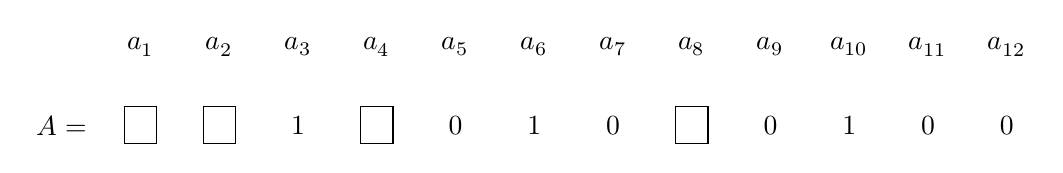
\begin{tikzpicture}
					\node[] (A) at (0,0) {$A = $};
					\node[draw, right of = A] (a01) at (0,0)        {\phantom{1}};
					\node[draw, right of = a01] (a02) {\phantom{1}};
					\node[right of = a02] (a03) {1};
					\node[draw, right of = a03] (a04) {\phantom{1}};
					\node[right of = a04] (a05) {0};
					\node[right of = a05] (a06) {1};
					\node[right of = a06] (a07) {0};
					\node[draw, right of = a07] (a08) {\phantom{1}};
					\node[right of = a08] (a09) {0};
					\node[right of = a09] (a10) {1};
					\node[right of = a10] (a11) {0};
					\node[right of = a11] (a12) {0};

					\node[above of = a01] (a01_t) {$a_{1}$};
					\node[above of = a02] (a02_t) {$a_{2}$};
					\node[above of = a03] (a03_t) {$a_{3}$};
					\node[above of = a04] (a04_t) {$a_{4}$};
					\node[above of = a05] (a05_t) {$a_{5}$};
					\node[above of = a06] (a06_t) {$a_{6}$};
					\node[above of = a07] (a07_t) {$a_{7}$};
					\node[above of = a08] (a08_t) {$a_{8}$};
					\node[above of = a09] (a09_t) {$a_{9}$};
					\node[above of = a10] (a10_t) {$a_{10}$};
					\node[above of = a11] (a11_t) {$a_{11}$};
					\node[above of = a12] (a12_t) {$a_{12}$};
				\end{tikzpicture}
			\]

			Щоб знайти значення контрольного розряду, необхідно обчислити суму по~модулю~2~(позначається~$\oplus$) усіх розрядів, які він покриває. Щоб визначити розряди, які покриває контрольний розряд, зобразимо порядкові номери~$i$ розрядів слова~$A$ у~десятковій та двійковій системах числення~(табл.~\ref{tab:01-word-a-bit-numbers}). До контрольної групи~$C_j$ ввійдуть ті розряди, в~яких біт~$i_j = 1$.

			\begin{table}[!htbp]
				\centering
				\caption{Номер розряду~$i$ слова~$A$ у двійковій та десятковій системах числення}
				\label{tab:01-word-a-bit-numbers}
				\begin{tabular}{
						v{3\gridunitwidth - 2\tabcolsep}
						n{1\gridunitwidth - 2\tabcolsep}
						n{1\gridunitwidth - 2\tabcolsep}
						n{1\gridunitwidth - 2\tabcolsep}
						n{1\gridunitwidth - 2\tabcolsep}
				}
					\toprule
						 & \multicolumn{4}{r}{$i_{\text{bin}}$}\\
						\cmidrule(lr){2-5}
						$i_{\text{dec}}$ & $i_4$ & $i_3$ & $i_2$ & $i_1$\\
					\midrule
						1  & 0 & 0 & 0 & 1\\
						2  & 0 & 0 & 1 & 0\\
						3  & 0 & 0 & 1 & 1\\
						4  & 0 & 1 & 0 & 0\\
						5  & 0 & 1 & 0 & 1\\
						6  & 0 & 1 & 1 & 0\\
						7  & 0 & 1 & 1 & 1\\
						8  & 1 & 0 & 0 & 0\\
						9  & 1 & 0 & 0 & 1\\
						10 & 1 & 0 & 1 & 0\\
						11 & 1 & 0 & 1 & 1\\
						12 & 1 & 1 & 0 & 0\\
					\midrule
						Контрольна група (якщо $i_j = 1$) & $C_4$ & $C_3$ & $C_2$ & $C_1$\\
					\bottomrule
				\end{tabular}
			\end{table}

			Розглянувши двійкове представлення індексів розрядів~(табл.~\ref{tab:01-word-a-bit-numbers}), визначили приналежність розрядів до~кожної контрольної групи:
			\begin{IEEEeqnarray*}{rCl}
				C_1 &=& \{a_1, a_3, a_5, a_7, a_9, a_{11}\},\\
				C_2 &=& \{a_2, a_3, a_6, a_7, a_{10}, a_{11}\},\\
				C_3 &=& \{a_4, a_5, a_6, a_7, a_{12}\},\\
				C_4 &=& \{a_8, a_9, a_{10}, a_{11}, a_{12}\}.
			\end{IEEEeqnarray*}
			Обчислимо контрольні розряди кожної контрольної групи, вважаючи значення пустих контрольних розрядів за~0:
			\begin{IEEEeqnarray*}{rClCl}
				C_1 &\mapsto& a_1 &=& a_1 \oplus a_3 \oplus a_5 \oplus a_7 \oplus a_9 \oplus a_{11} = 0 \oplus 1 \oplus 0 \oplus 0 \oplus 0 \oplus 0 = 1,\\
				C_2 &\mapsto& a_2 &=& a_2 \oplus a_3 \oplus a_6 \oplus a_7 \oplus a_{10} \oplus a_{11} = 0 \oplus 1 \oplus 1 \oplus 0 \oplus 1 \oplus 0 = 1,\\
				C_3 &\mapsto& a_4 &=& a_4 \oplus a_5 \oplus a_6 \oplus a_7 \oplus a_{12} = 0 \oplus 0 \oplus 1 \oplus 0 \oplus 0 = 1,\\
				C_4 &\mapsto& a_8 &=& a_8 \oplus a_9 \oplus a_{10} \oplus a_{11} \oplus a_{12} = 0 \oplus 0 \oplus 1 \oplus 0 \oplus 0 = 1.
			\end{IEEEeqnarray*}
			Впишемо знайдені контрольні розряди:
			\[
				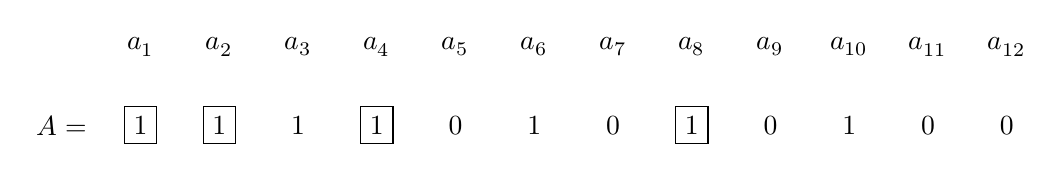
\begin{tikzpicture}
					\node[] (A) at (0,0) {$A = $};
					\node[draw, right of = A] (a01) {1};
					\node[draw, right of = a01] (a02) {1};
					\node[right of = a02] (a03) {1};
					\node[draw, right of = a03] (a04) {1};
					\node[right of = a04] (a05) {0};
					\node[right of = a05] (a06) {1};
					\node[right of = a06] (a07) {0};
					\node[draw, right of = a07] (a08) {1};
					\node[right of = a08] (a09) {0};
					\node[right of = a09] (a10) {1};
					\node[right of = a10] (a11) {0};
					\node[right of = a11] (a12) {0};

					\node[above of = a01] (a01_t) {$a_{1}$};
					\node[above of = a02] (a02_t) {$a_{2}$};
					\node[above of = a03] (a03_t) {$a_{3}$};
					\node[above of = a04] (a04_t) {$a_{4}$};
					\node[above of = a05] (a05_t) {$a_{5}$};
					\node[above of = a06] (a06_t) {$a_{6}$};
					\node[above of = a07] (a07_t) {$a_{7}$};
					\node[above of = a08] (a08_t) {$a_{8}$};
					\node[above of = a09] (a09_t) {$a_{9}$};
					\node[above of = a10] (a10_t) {$a_{10}$};
					\node[above of = a11] (a11_t) {$a_{11}$};
					\node[above of = a12] (a12_t) {$a_{12}$};
				\end{tikzpicture}
			\]
			Таким чином ми отримали слово~$A = 111101001100_{\text{bin}}$, закодувавши задане число~$N$ кодом Хемінга.

			Для перевірки правильності кодування необхідно обчислити суму по модулю 2 для кожної контрольної групи. Якщо кодування виконано правильно, кожна сума~$s_i$ повинна дорівнювати 0. Виконуємо обчислення:
			\begin{IEEEeqnarray*}{rCl}
				s_1 &=& a_1 \oplus a_3 \oplus a_5 \oplus a_7 \oplus a_9 \oplus a_{11} = 1 \oplus 1 \oplus 0 \oplus 0 \oplus 0 \oplus 0 = 0,\\
				s_2 &=& a_2 \oplus a_3 \oplus a_6 \oplus a_7 \oplus a_{10} \oplus a_{11} = 1 \oplus 1 \oplus 1 \oplus 0 \oplus 1 \oplus 0 = 0,\\
				s_3 &=& a_4 \oplus a_5 \oplus a_6 \oplus a_7 \oplus a_{12} = 1 \oplus 0 \oplus 1 \oplus 0 \oplus 0 = 0,\\
				s_4 &=& a_8 \oplus a_9 \oplus a_{10} \oplus a_{11} \oplus a_{12} = 1 \oplus 0 \oplus 1 \oplus 0 \oplus 0 = 0.
			\end{IEEEeqnarray*}
			Як бачимо, усі суми дорівнюють 0, тому кодування виконано правильно.

		\subsection{Формування посиленого коду Хемінга}
		\label{ssec:hamming-code-secded}
			Нехай слово~$B$~— результат кодування заданого числа~$N$ посиленим кодом Хемінга. Оскільки принцип посиленого кодування Хемінга аналогічний простому, щоб сформувати слово~$B$ для заданого числа~$N$, до слова~$A$~(пп.~\ref{ssec:hamming-code-sec}) додаємо розряд~$b_{13}$, який міститиме загальний біт парності~$p$. Значення~$p$ буде сумою по~модулю~2 усіх розрядів слова:
			\[
				b_{13} = p = \bigoplus_{i = 1}^{12} b_i = 1.
			\]
			Вписуємо отримане значення~$b_{13}$:
			\[
				\begin{tikzpicture}
					\node[] (B) at (0,0) {$B = $};
					\node[draw, right of = B] (b01) {1};
					\node[draw, right of = a01] (b02) {1};
					\node[right of = b02] (b03) {1};
					\node[draw, right of = b03] (b04) {1};
					\node[right of = b04] (b05) {0};
					\node[right of = b05] (b06) {1};
					\node[right of = b06] (b07) {0};
					\node[draw, right of = b07] (b08) {1};
					\node[right of = b08] (b09) {0};
					\node[right of = b09] (b10) {1};
					\node[right of = b10] (b11) {0};
					\node[right of = b11] (b12) {0};
					\node[draw, right of = b12] (b13) {1};

					\node[above of = b01] (b01_t) {$b_{1}$};
					\node[above of = b02] (b02_t) {$b_{2}$};
					\node[above of = b03] (b03_t) {$b_{3}$};
					\node[above of = b04] (b04_t) {$b_{4}$};
					\node[above of = b05] (b05_t) {$b_{5}$};
					\node[above of = b06] (b06_t) {$b_{6}$};
					\node[above of = b07] (b07_t) {$b_{7}$};
					\node[above of = b08] (b08_t) {$b_{8}$};
					\node[above of = b09] (b09_t) {$b_{9}$};
					\node[above of = b10] (b10_t) {$b_{10}$};
					\node[above of = b11] (b11_t) {$b_{11}$};
					\node[above of = b12] (b12_t) {$b_{12}$};
					\node[above of = b13] (b13_t) {$b_{13}$};
				\end{tikzpicture}
			\]
			Таким чином ми сформували слово~$B$, яке містить задане число~$N$, закодоване посиленим кодом Хемінга. Таке кодування дозволяє коригувати 1~помилку та~виявляти~2.

		\subsection{Декодування та емуляція передачі}
			При передачі даних приймається слово, закодоване одним з кодів Хемінга, його контрольні розряди відкидаються та обчислюються заново за тим же алгоритмом, яким проводилось кодування (описані в~пп.~\ref{ssec:hamming-code-sec}, \ref{ssec:hamming-code-secded}). В залежності від результату обчислення та його відповідності отриманим контрольним розрядам робиться висновок, чи були дані передані правильно.
			
			\subsubsection{Для простого коду Хемінга}
			\label{sssec:hamming-code-decode-sec}
				Припустимо, що передавач відправив слово~$C$, а~приймач отримав слово~$C'$. Число~$S'$ складається з контрольних розрядів слова~$C'$, як вони і були отримані; число~$S''$~— з контрольних розрядів, заново обчислених приймачем з розрядів даних. Для виявлення помилки обчислюється синдром~$E$:
				\[
					E = S' \oplus S''.
				\]
				Якщо $E = 0$, тобто всі контрольні розряди співпадають, помилки при передачі не виявлені і відсутні, якщо відбулось не більше 1 помилки. Якщо~$E$ містить лише один розряд~$e_i = 1$, тобто контрольні розряди відрізняються лише одним бітом, то при передачі виникла помилка лише в цьому контрольному розряді. В~інших випадках значення синдрому~$E$ буде вказувати на індекс розряду, в~якому відбулась помилка.

				Наприклад: нехай при передачі передавач відправив слово~$A$~(пп.~\ref{ssec:hamming-code-sec}):
				\[
					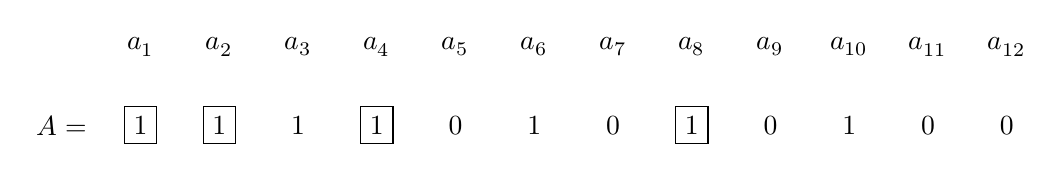
\begin{tikzpicture}
						\node[] (A) at (0,0) {$A = $};
						\node[draw, right of = A] (a01) {1};
						\node[draw, right of = a01] (a02) {1};
						\node[right of = a02] (a03) {1};
						\node[draw, right of = a03] (a04) {1};
						\node[right of = a04] (a05) {0};
						\node[right of = a05] (a06) {1};
						\node[right of = a06] (a07) {0};
						\node[draw, right of = a07] (a08) {1};
						\node[right of = a08] (a09) {0};
						\node[right of = a09] (a10) {1};
						\node[right of = a10] (a11) {0};
						\node[right of = a11] (a12) {0};

						\node[above of = a01] (a01_t) {$a_{1}$};
						\node[above of = a02] (a02_t) {$a_{2}$};
						\node[above of = a03] (a03_t) {$a_{3}$};
						\node[above of = a04] (a04_t) {$a_{4}$};
						\node[above of = a05] (a05_t) {$a_{5}$};
						\node[above of = a06] (a06_t) {$a_{6}$};
						\node[above of = a07] (a07_t) {$a_{7}$};
						\node[above of = a08] (a08_t) {$a_{8}$};
						\node[above of = a09] (a09_t) {$a_{9}$};
						\node[above of = a10] (a10_t) {$a_{10}$};
						\node[above of = a11] (a11_t) {$a_{11}$};
						\node[above of = a12] (a12_t) {$a_{12}$};
					\end{tikzpicture}
				\]
				Приймач отримав слово~$A'$, і~відбулась 1~помилка у~розряді~$a'_5$~(тут і~далі помилкові розряди позначаються колом). Тоді отримане слово~$A'$ виглядатиме так:
				\[
					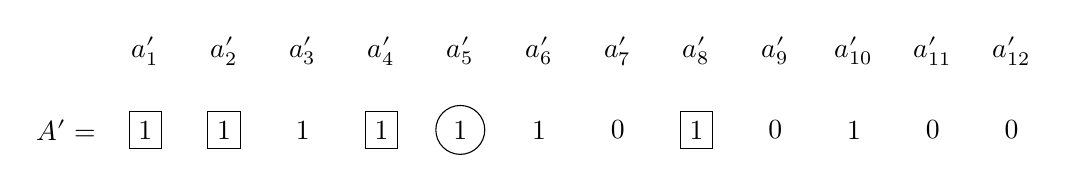
\begin{tikzpicture}
						\node[] (A-prime) at (0,0) {$A' = $};
						\node[draw, right of = A-prime] (a01) {1};
						\node[draw, right of = a01] (a02) {1};
						\node[right of = a02] (a03) {1};
						\node[draw, right of = a03] (a04) {1};
						\node[draw, circle, right of = a04] (a05) {1};
						\node[right of = a05] (a06) {1};
						\node[right of = a06] (a07) {0};
						\node[draw, right of = a07] (a08) {1};
						\node[right of = a08] (a09) {0};
						\node[right of = a09] (a10) {1};
						\node[right of = a10] (a11) {0};
						\node[right of = a11] (a12) {0};

						\node[above of = a01] (a01_t) {$a'_{1}$};
						\node[above of = a02] (a02_t) {$a'_{2}$};
						\node[above of = a03] (a03_t) {$a'_{3}$};
						\node[above of = a04] (a04_t) {$a'_{4}$};
						\node[above of = a05] (a05_t) {$a'_{5}$};
						\node[above of = a06] (a06_t) {$a'_{6}$};
						\node[above of = a07] (a07_t) {$a'_{7}$};
						\node[above of = a08] (a08_t) {$a'_{8}$};
						\node[above of = a09] (a09_t) {$a'_{9}$};
						\node[above of = a10] (a10_t) {$a'_{10}$};
						\node[above of = a11] (a11_t) {$a'_{11}$};
						\node[above of = a12] (a12_t) {$a'_{12}$};
					\end{tikzpicture}
				\]

				Запишемо заново обчислюване слово~$A''$, відкинувши отримані контрольні розряди:
				\[
					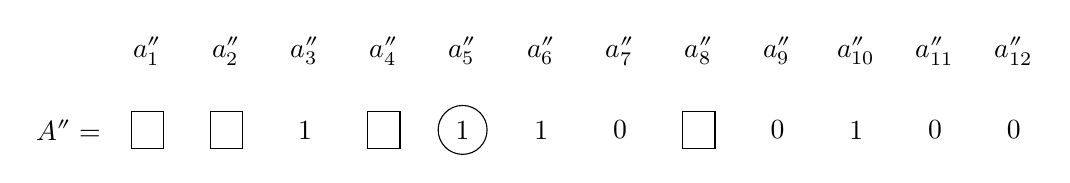
\begin{tikzpicture}
						\node[] (A-dbl-prime) at (0,0) {$A'' = $};
						\node[draw, right of = A-dbl-prime] (a01) {\phantom{1}};
						\node[draw, right of = a01] (a02) {\phantom{1}};
						\node[right of = a02] (a03) {1};
						\node[draw, right of = a03] (a04) {\phantom{1}};
						\node[draw, circle, right of = a04] (a05) {1};
						\node[right of = a05] (a06) {1};
						\node[right of = a06] (a07) {0};
						\node[draw, right of = a07] (a08) {\phantom{1}};
						\node[right of = a08] (a09) {0};
						\node[right of = a09] (a10) {1};
						\node[right of = a10] (a11) {0};
						\node[right of = a11] (a12) {0};

						\node[above of = a01] (a01_t) {$a''_{1}$};
						\node[above of = a02] (a02_t) {$a''_{2}$};
						\node[above of = a03] (a03_t) {$a''_{3}$};
						\node[above of = a04] (a04_t) {$a''_{4}$};
						\node[above of = a05] (a05_t) {$a''_{5}$};
						\node[above of = a06] (a06_t) {$a''_{6}$};
						\node[above of = a07] (a07_t) {$a''_{7}$};
						\node[above of = a08] (a08_t) {$a''_{8}$};
						\node[above of = a09] (a09_t) {$a''_{9}$};
						\node[above of = a10] (a10_t) {$a''_{10}$};
						\node[above of = a11] (a11_t) {$a''_{11}$};
						\node[above of = a12] (a12_t) {$a''_{12}$};
					\end{tikzpicture}
				\]

				Обчислюємо контрольні розряди слова~$A''$ за отриманими розрядами даних:
				\begin{IEEEeqnarray*}{rCl}
					a''_{1} &=& a''_1 \oplus a''_3 \oplus a''_5 \oplus a''_7 \oplus a''_9 \oplus a''_{11} = 0,\\
					a''_{2} &=& a''_2 \oplus a''_3 \oplus a''_6 \oplus a''_7 \oplus a''_{10} \oplus a''_{11} = 1,\\
					a''_{4} &=& a''_4 \oplus a''_5 \oplus a''_6 \oplus a''_7 \oplus a''_{12} = 0,\\
					a''_{8} &=& a''_8 \oplus a''_9 \oplus a''_{10} \oplus a''_{11} \oplus a''_{12} = 1.
				\end{IEEEeqnarray*}

				Вписуємо обчислені контрольні розряди слова~$A''$:
				\[
					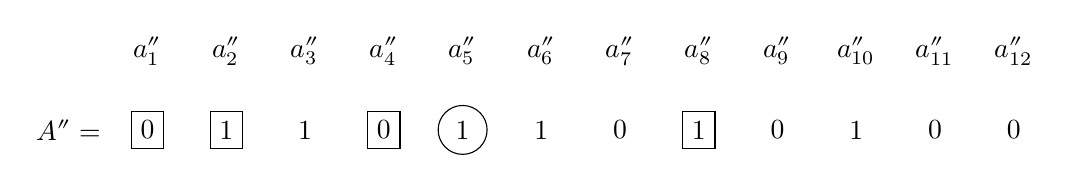
\begin{tikzpicture}
						\node[] (A-dbl-prime) at (0,0) {$A'' = $};
						\node[draw, right of = A-dbl-prime] (a01) {0};
						\node[draw, right of = a01] (a02) {1};
						\node[right of = a02] (a03) {1};
						\node[draw, right of = a03] (a04) {0};
						\node[draw, circle, right of = a04] (a05) {1};
						\node[right of = a05] (a06) {1};
						\node[right of = a06] (a07) {0};
						\node[draw, right of = a07] (a08) {1};
						\node[right of = a08] (a09) {0};
						\node[right of = a09] (a10) {1};
						\node[right of = a10] (a11) {0};
						\node[right of = a11] (a12) {0};

						\node[above of = a01] (a01_t) {$a''_{1}$};
						\node[above of = a02] (a02_t) {$a''_{2}$};
						\node[above of = a03] (a03_t) {$a''_{3}$};
						\node[above of = a04] (a04_t) {$a''_{4}$};
						\node[above of = a05] (a05_t) {$a''_{5}$};
						\node[above of = a06] (a06_t) {$a''_{6}$};
						\node[above of = a07] (a07_t) {$a''_{7}$};
						\node[above of = a08] (a08_t) {$a''_{8}$};
						\node[above of = a09] (a09_t) {$a''_{9}$};
						\node[above of = a10] (a10_t) {$a''_{10}$};
						\node[above of = a11] (a11_t) {$a''_{11}$};
						\node[above of = a12] (a12_t) {$a''_{12}$};
					\end{tikzpicture}
				\]

				Таким чином отримані числа~$S' = 1111$ та~$S'' = 0101$, з їх допомогою обчислюємо розряди синдрому~$e_1, e_2, e_3, e_4$:
				\begin{IEEEeqnarray*}{rCl}
					e_1 = a''_8 \oplus a'_8 &=& 1 \oplus 1 = 0,\\
					e_2 = a''_4 \oplus a'_4 &=& 0 \oplus 1 = 1,\\
					e_3 = a''_2 \oplus a'_2 &=& 1 \oplus 1 = 0,\\
					e_4 = a''_1 \oplus a'_1 &=& 0 \oplus 1 = 1.
				\end{IEEEeqnarray*}
				З обчислених значень розрядів синдрому складаємо його значення~$E = 0101_{\text{bin}} = 5_{\text{dec}}$, що вказує на помилку у розряді~$a'_5$. Для її виправлення достатньо змінити значення помилкового розряду~$a'_5$.

			\subsubsection{Для посиленого коду Хемінга}
			\label{sssec:hamming-code-decode-secded}
				Алгоритм декодування та перевірки помилок для посиленого коду Хемінга аналогічний простому~(ппп.~\ref{sssec:hamming-code-decode-sec}), але внесення додаткового загального розряду парності~$p$ вносить особливості інтерпретації контрольних розрядів~(табл.~\ref{tab:hamming-code-secded-meanings}).

				\begin{table}[!htbp]
					\centering
					\caption{Виявлення помилок у посиленому коді Хемінга; $E$~— синдром, $p$~— загальний біт парності}
					\label{tab:hamming-code-secded-meanings}
					\begin{tabular}{
							n{1\gridunitwidth - 2\tabcolsep}
							n{1\gridunitwidth - 2\tabcolsep}
							v{4\gridunitwidth - 2\tabcolsep}
							v{6\gridunitwidth - 2\tabcolsep}
					}
						\toprule
							$E$ & $p$ & Тип помилки & Опис\\
						\midrule
						$0$ & 0 & Немає & При передачі помилки не відбулось\\
						${\neq} 0$ & 1 & Одиночна & Помилку можна виправити: у~синдромі зберігається позиція помилкового розряду\\
						${\neq} 0$ & 0 & Подвійна & Помилку неможливо виправити\\
						$0$ & 1 & Парність & Помилка виникла лише у~загальному біті парності~$p$, її можна виправити\\
						\bottomrule
					\end{tabular}
				\end{table}
				
				Наприклад: нехай при передачі передавач відправив слово~$B$~(пп.~\ref{ssec:hamming-code-secded}):
				\[
					\begin{tikzpicture}
						\node[] (B) at (0,0) {$B = $};
						\node[draw, right of = B] (b01) {1};
						\node[draw, right of = a01] (b02) {1};
						\node[right of = b02] (b03) {1};
						\node[draw, right of = b03] (b04) {1};
						\node[right of = b04] (b05) {0};
						\node[right of = b05] (b06) {1};
						\node[right of = b06] (b07) {0};
						\node[draw, right of = b07] (b08) {1};
						\node[right of = b08] (b09) {0};
						\node[right of = b09] (b10) {1};
						\node[right of = b10] (b11) {0};
						\node[right of = b11] (b12) {0};
						\node[draw, right of = b12] (b13) {1};

						\node[above of = b01] (b01_t) {$b_{1}$};
						\node[above of = b02] (b02_t) {$b_{2}$};
						\node[above of = b03] (b03_t) {$b_{3}$};
						\node[above of = b04] (b04_t) {$b_{4}$};
						\node[above of = b05] (b05_t) {$b_{5}$};
						\node[above of = b06] (b06_t) {$b_{6}$};
						\node[above of = b07] (b07_t) {$b_{7}$};
						\node[above of = b08] (b08_t) {$b_{8}$};
						\node[above of = b09] (b09_t) {$b_{9}$};
						\node[above of = b10] (b10_t) {$b_{10}$};
						\node[above of = b11] (b11_t) {$b_{11}$};
						\node[above of = b12] (b12_t) {$b_{12}$};
						\node[above of = b13] (b13_t) {$b_{13}$};
					\end{tikzpicture}
				\]
				Приймач отримав слово~$B'$, і~виникло 2~помилки: у~розрядах~$b'_5$ і~$b'_{10}$. Тоді отримане слово~$B'$ виглядатиме так:
			\[
				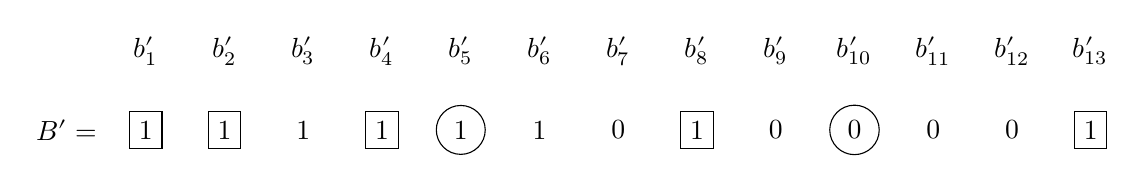
\begin{tikzpicture}
					\node[] (B-prime) at (0,0) {$B' = $};
					\node[draw, right of = B-prime] (b01) {1};
					\node[draw, right of = b01] (b02) {1};
					\node[right of = b02] (b03) {1};
					\node[draw, right of = b03] (b04) {1};
					\node[draw, circle ,right of = b04] (b05) {1};
					\node[right of = b05] (b06) {1};
					\node[right of = b06] (b07) {0};
					\node[draw, right of = b07] (b08) {1};
					\node[right of = b08] (b09) {0};
					\node[draw, circle, right of = b09] (b10) {0};
					\node[right of = b10] (b11) {0};
					\node[right of = b11] (b12) {0};
					\node[draw, right of = b12] (b13) {1};

					\node[above of = b01] (b01_t) {$b'_{1}$};
					\node[above of = b02] (b02_t) {$b'_{2}$};
					\node[above of = b03] (b03_t) {$b'_{3}$};
					\node[above of = b04] (b04_t) {$b'_{4}$};
					\node[above of = b05] (b05_t) {$b'_{5}$};
					\node[above of = b06] (b06_t) {$b'_{6}$};
					\node[above of = b07] (b07_t) {$b'_{7}$};
					\node[above of = b08] (b08_t) {$b'_{8}$};
					\node[above of = b09] (b09_t) {$b'_{9}$};
					\node[above of = b10] (b10_t) {$b'_{10}$};
					\node[above of = b11] (b11_t) {$b'_{11}$};
					\node[above of = b12] (b12_t) {$b'_{12}$};
					\node[above of = b13] (b13_t) {$b'_{13}$};
				\end{tikzpicture}
			\]

			Запишемо заново обчислюване слово~$B''$, відкинувши отримані контрольні розряди:
			\[
				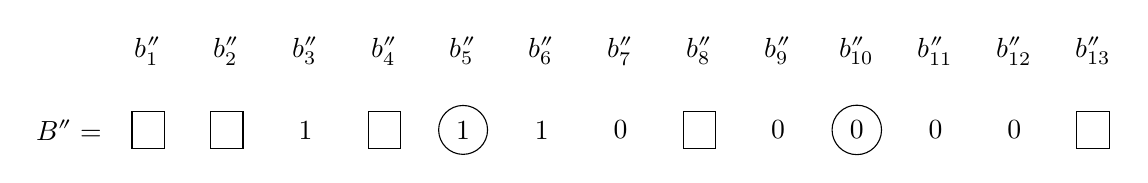
\begin{tikzpicture}
					\node[] (B-dbl-prime) at (0,0) {$B'' = $};
					\node[draw, right of = B-dbl-prime] (b01) {\phantom{1}};
					\node[draw, right of = b01] (b02) {\phantom{1}};
					\node[right of = b02] (b03) {1};
					\node[draw, right of = b03] (b04) {\phantom{1}};
					\node[draw, circle, right of = b04] (b05) {1};
					\node[right of = b05] (b06) {1};
					\node[right of = b06] (b07) {0};
					\node[draw, right of = b07] (b08) {\phantom{1}};
					\node[right of = b08] (b09) {0};
					\node[draw, circle, right of = b09] (b10) {0};
					\node[right of = b10] (b11) {0};
					\node[right of = b11] (b12) {0};
					\node[draw, right of = b12] (b13) {\phantom{1}};

					\node[above of = b01] (b01_t) {$b''_{1}$};
					\node[above of = b02] (b02_t) {$b''_{2}$};
					\node[above of = b03] (b03_t) {$b''_{3}$};
					\node[above of = b04] (b04_t) {$b''_{4}$};
					\node[above of = b05] (b05_t) {$b''_{5}$};
					\node[above of = b06] (b06_t) {$b''_{6}$};
					\node[above of = b07] (b07_t) {$b''_{7}$};
					\node[above of = b08] (b08_t) {$b''_{8}$};
					\node[above of = b09] (b09_t) {$b''_{9}$};
					\node[above of = b10] (b10_t) {$b''_{10}$};
					\node[above of = b11] (b11_t) {$b''_{11}$};
					\node[above of = b12] (b12_t) {$b''_{12}$};
					\node[above of = b13] (b13_t) {$b''_{13}$};
				\end{tikzpicture}
			\]

			Обчислюємо контрольні розряди~$b''_1, b''_2, b''_3, b''_4$ слова~$B''$ за~отриманими розрядами даних (загальний біт парності~$p = b_{13}$ при розрахунках контрольних розрядів не враховується):
				\begin{IEEEeqnarray*}{rCl}
					b''_{1} &=& b''_1 \oplus b''_3 \oplus b''_5 \oplus b''_7 \oplus b''_9 \oplus b''_{11} = 0 \oplus 1 \oplus 1 \oplus 0 \oplus 0 \oplus 0 = 0,\\
					b''_{2} &=& b''_2 \oplus b''_3 \oplus b''_6 \oplus b''_7 \oplus b''_{10} \oplus b''_{11} = 0 \oplus 1 \oplus 1 \oplus 0 \oplus 0 \oplus 0 = 0,\\
					b''_{4} &=& b''_4 \oplus b''_5 \oplus b''_6 \oplus b''_7 \oplus b''_{12} = 0 \oplus 1 \oplus 1 \oplus 0 \oplus 0 = 0,\\
					b''_{8} &=& b''_8 \oplus b''_9 \oplus b''_{10} \oplus b''_{11} \oplus b''_{12} = 0 \oplus 0 \oplus 0 \oplus 0 \oplus 0 = 0.
				\end{IEEEeqnarray*}

			Вписуємо обчислені контрольні розряди~$b''_1, b''_2, b''_3, b''_4$:
			\[
				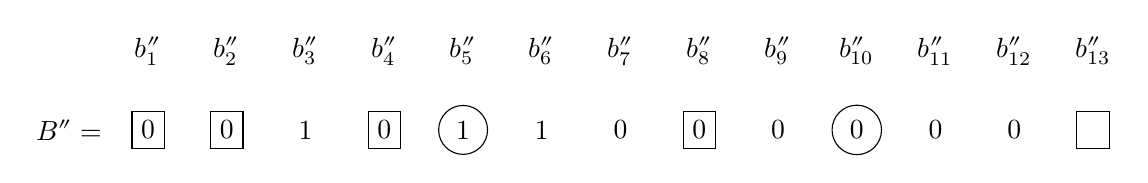
\begin{tikzpicture}
					\node[] (B-dbl-prime) at (0,0) {$B'' = $};
					\node[draw, right of = B-dbl-prime] (b01) {0};
					\node[draw, right of = b01] (b02) {0};
					\node[right of = b02] (b03) {1};
					\node[draw, right of = b03] (b04) {0};
					\node[draw, circle, right of = b04] (b05) {1};
					\node[right of = b05] (b06) {1};
					\node[right of = b06] (b07) {0};
					\node[draw, right of = b07] (b08) {0};
					\node[right of = b08] (b09) {0};
					\node[draw, circle, right of = b09] (b10) {0};
					\node[right of = b10] (b11) {0};
					\node[right of = b11] (b12) {0};
					\node[draw, right of = b12] (b13) {\phantom{1}};

					\node[above of = b01] (b01_t) {$b''_{1}$};
					\node[above of = b02] (b02_t) {$b''_{2}$};
					\node[above of = b03] (b03_t) {$b''_{3}$};
					\node[above of = b04] (b04_t) {$b''_{4}$};
					\node[above of = b05] (b05_t) {$b''_{5}$};
					\node[above of = b06] (b06_t) {$b''_{6}$};
					\node[above of = b07] (b07_t) {$b''_{7}$};
					\node[above of = b08] (b08_t) {$b''_{8}$};
					\node[above of = b09] (b09_t) {$b''_{9}$};
					\node[above of = b10] (b10_t) {$b''_{10}$};
					\node[above of = b11] (b11_t) {$b''_{11}$};
					\node[above of = b12] (b12_t) {$b''_{12}$};
					\node[above of = b13] (b13_t) {$b''_{13}$};
				\end{tikzpicture}
			\]

			Обчислюємо загальний біт парності~$p = b''_{13}= \bigoplus_{i = 1}^{12} b''_i = 0$ та вписуємо його в обчислене слово~$B''$:
			\[
				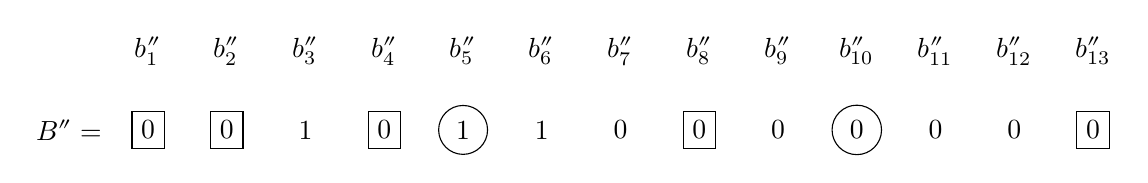
\begin{tikzpicture}
					\node[] (B-dbl-prime) at (0,0) {$B'' = $};
					\node[draw, right of = B-dbl-prime] (b01) {0};
					\node[draw, right of = b01] (b02) {0};
					\node[right of = b02] (b03) {1};
					\node[draw, right of = b03] (b04) {0};
					\node[draw, circle, right of = b04] (b05) {1};
					\node[right of = b05] (b06) {1};
					\node[right of = b06] (b07) {0};
					\node[draw, right of = b07] (b08) {0};
					\node[right of = b08] (b09) {0};
					\node[draw, circle, right of = b09] (b10) {0};
					\node[right of = b10] (b11) {0};
					\node[right of = b11] (b12) {0};
					\node[draw, right of = b12] (b13) {0};

					\node[above of = b01] (b01_t) {$b''_{1}$};
					\node[above of = b02] (b02_t) {$b''_{2}$};
					\node[above of = b03] (b03_t) {$b''_{3}$};
					\node[above of = b04] (b04_t) {$b''_{4}$};
					\node[above of = b05] (b05_t) {$b''_{5}$};
					\node[above of = b06] (b06_t) {$b''_{6}$};
					\node[above of = b07] (b07_t) {$b''_{7}$};
					\node[above of = b08] (b08_t) {$b''_{8}$};
					\node[above of = b09] (b09_t) {$b''_{9}$};
					\node[above of = b10] (b10_t) {$b''_{10}$};
					\node[above of = b11] (b11_t) {$b''_{11}$};
					\node[above of = b12] (b12_t) {$b''_{12}$};
					\node[above of = b13] (b13_t) {$b''_{13}$};
				\end{tikzpicture}
			\]

			Таким чином отримані числа~$S' = 1111$ та~$S'' = 0000$, з їх допомогою обчислюємо розряди синдрому~$e_1, e_2, e_3, e_4$:
				\begin{IEEEeqnarray*}{rClCl}
					e_1 &=& b''_8 \oplus b'_8 &=& 0 \oplus 1 = 1,\\
					e_2 &=& b''_4 \oplus b'_4 &=& 0 \oplus 1 = 1,\\
					e_3 &=& b''_2 \oplus b'_2 &=& 0 \oplus 1 = 1,\\
					e_4 &=& b''_1 \oplus b'_1 &=& 0 \oplus 1 = 1.
				\end{IEEEeqnarray*}
				Як бачимо, синдром~$E \neq 0$, і біт парності~$p = 0$, тому робимо висновок, що під час передачі сталась подвійна помилка, яку неможливо виправити.

	\section{Висновок}
		Виконуючи дану лабораторну роботу, ми~ознайомились з~методиками формування простого і~посиленого кодів Хемінга, а~також здобули практичні навички побудови кодів.


\end{document}
